\documentclass[../thesis.tex]{subfiles}
\begin{document}
\appendix
\chapter{Screenshots}\label{appendix:screenshot}
The frontend module provides three screens, each with specific tasks:

\autoref{fig:frontend_dashboard} allows the creation of new searches and the display of previous ones.

\autoref{fig:frontend_new_search} shows an overlay card that allows parameters to be entered for a new search.

\autoref{fig:frontend_search_details} allows all results of a specific search to be displayed and provides options for filtering them. As has already been mentioned, it will suffice to enter the keywords of interest within the HTML box to search them into the Elasticsearch index.

\begin{figure}[H]
    \centering
    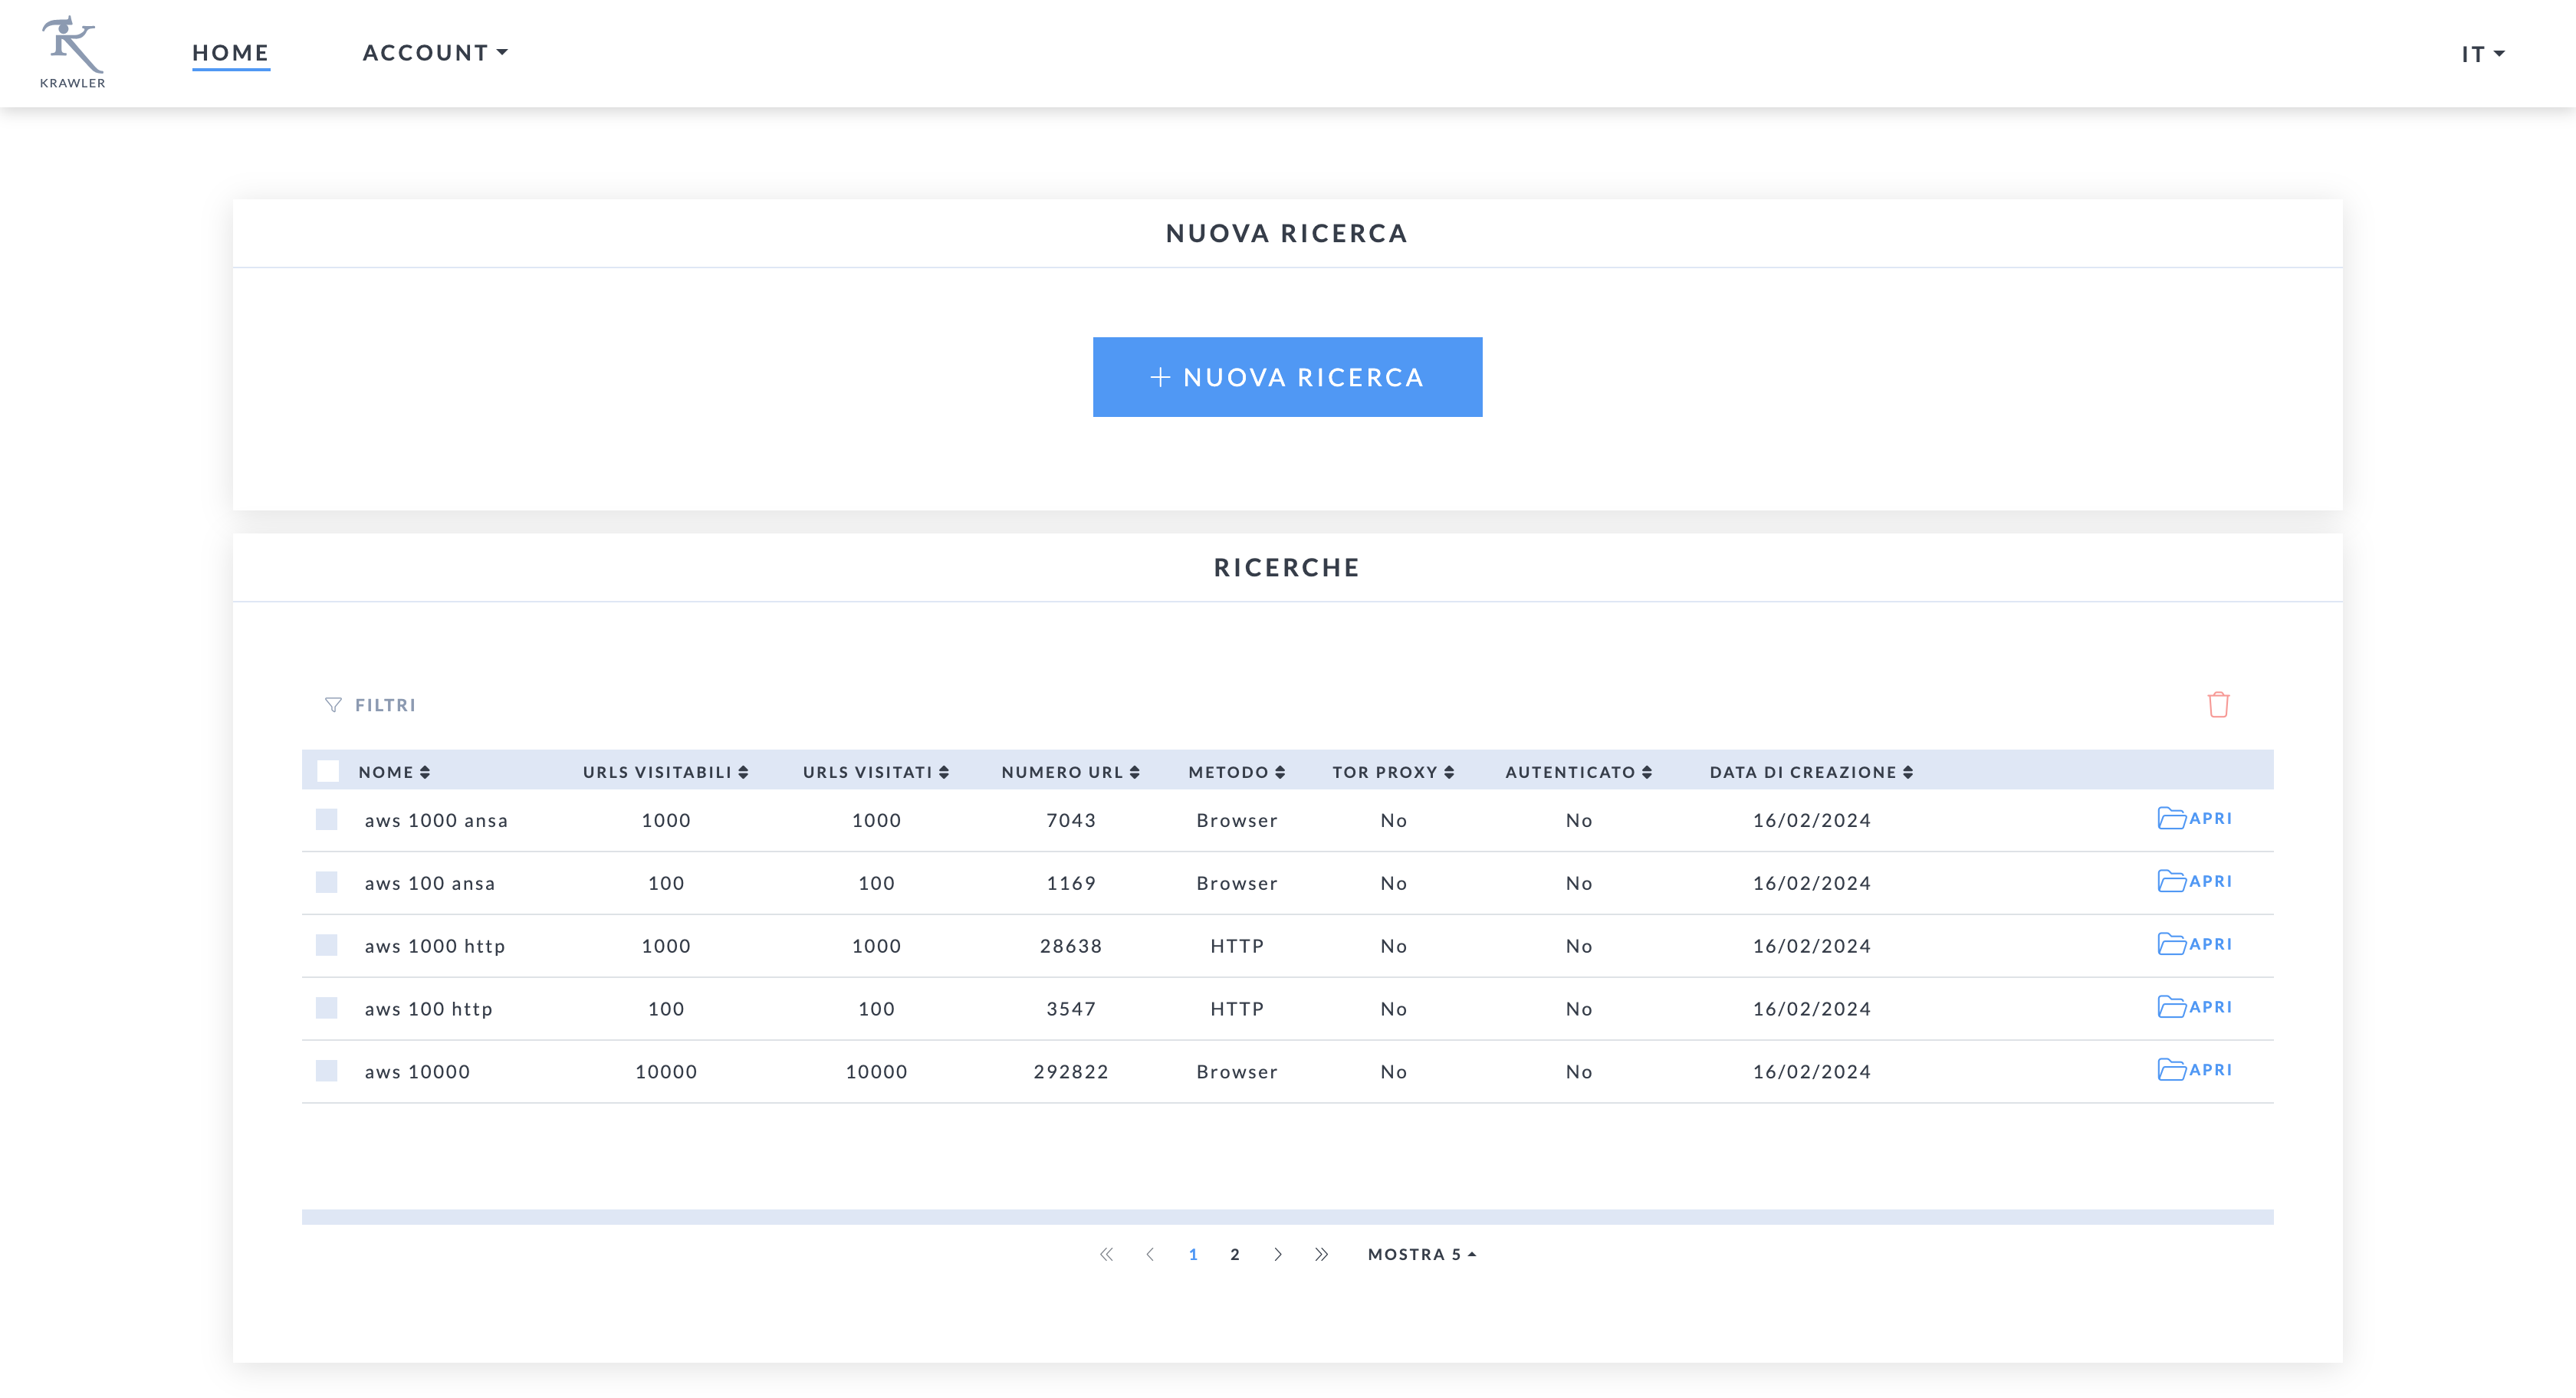
\includegraphics[width=1\textwidth]{appendix/frontend_dashboard.png}
    \caption[Dashboard screen]{Dashboard.}
    \label{fig:frontend_dashboard}
\end{figure}

\begin{figure}[H]
    \centering
    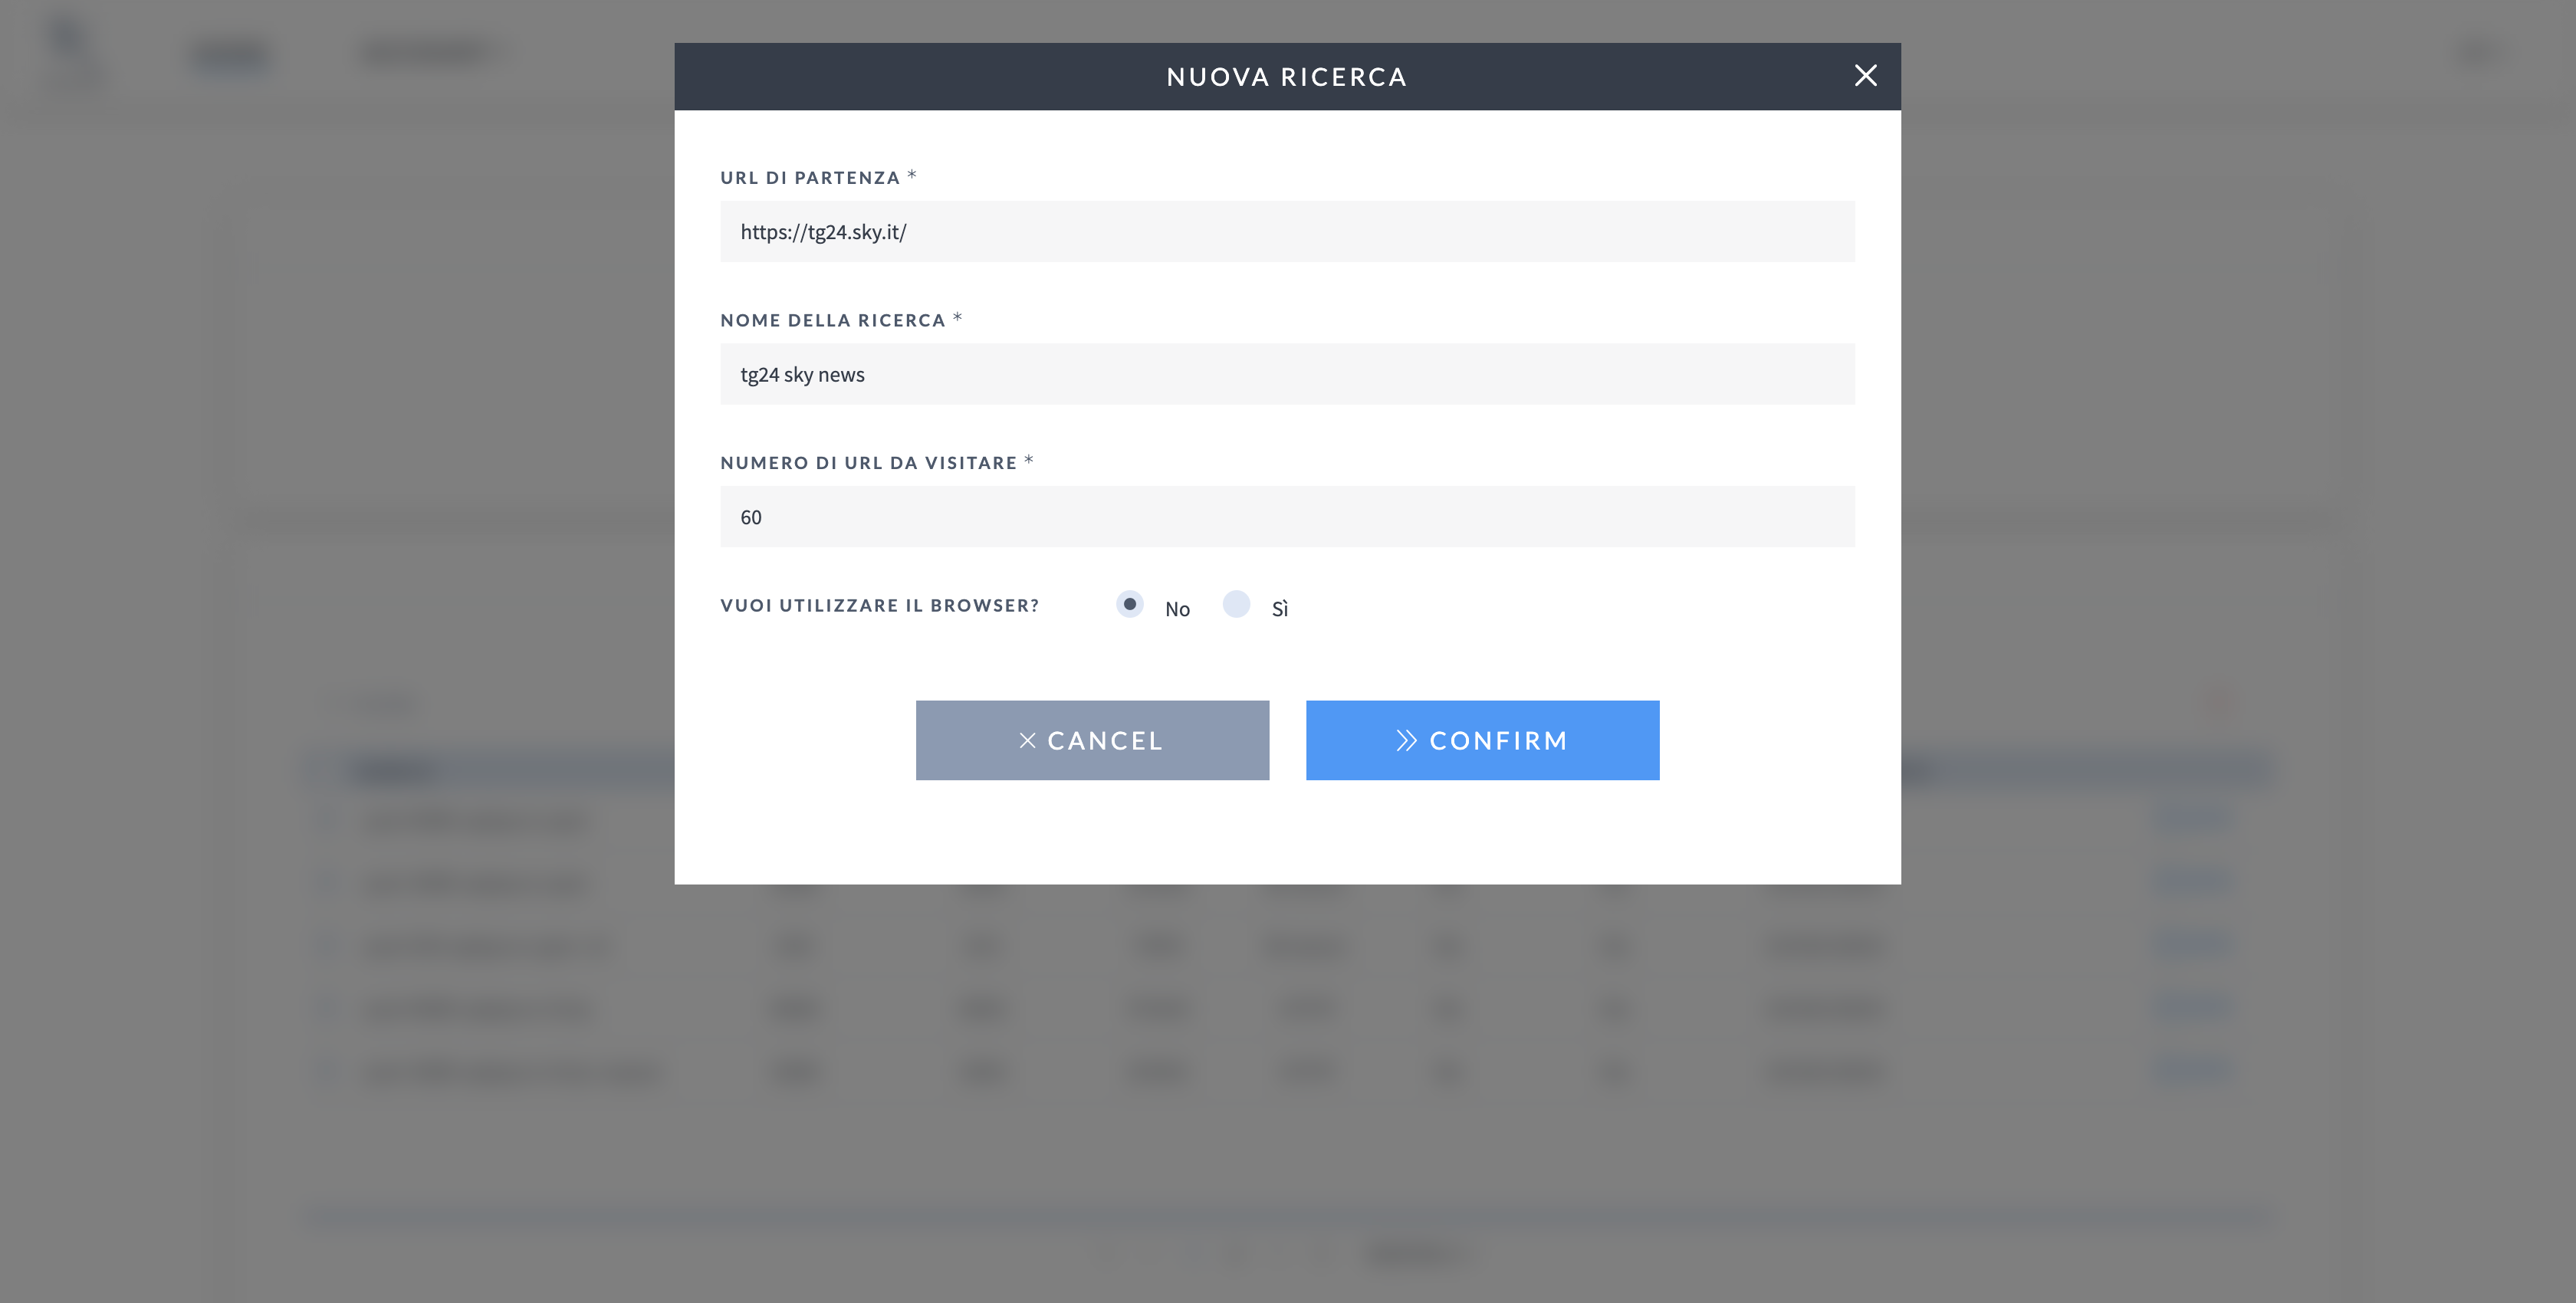
\includegraphics[width=1\textwidth]{appendix/frontend_new_search.png}
    \caption[New search creation screen]{Create a new search.}
    \label{fig:frontend_new_search}
\end{figure}

\begin{figure}[H]
    \centering
    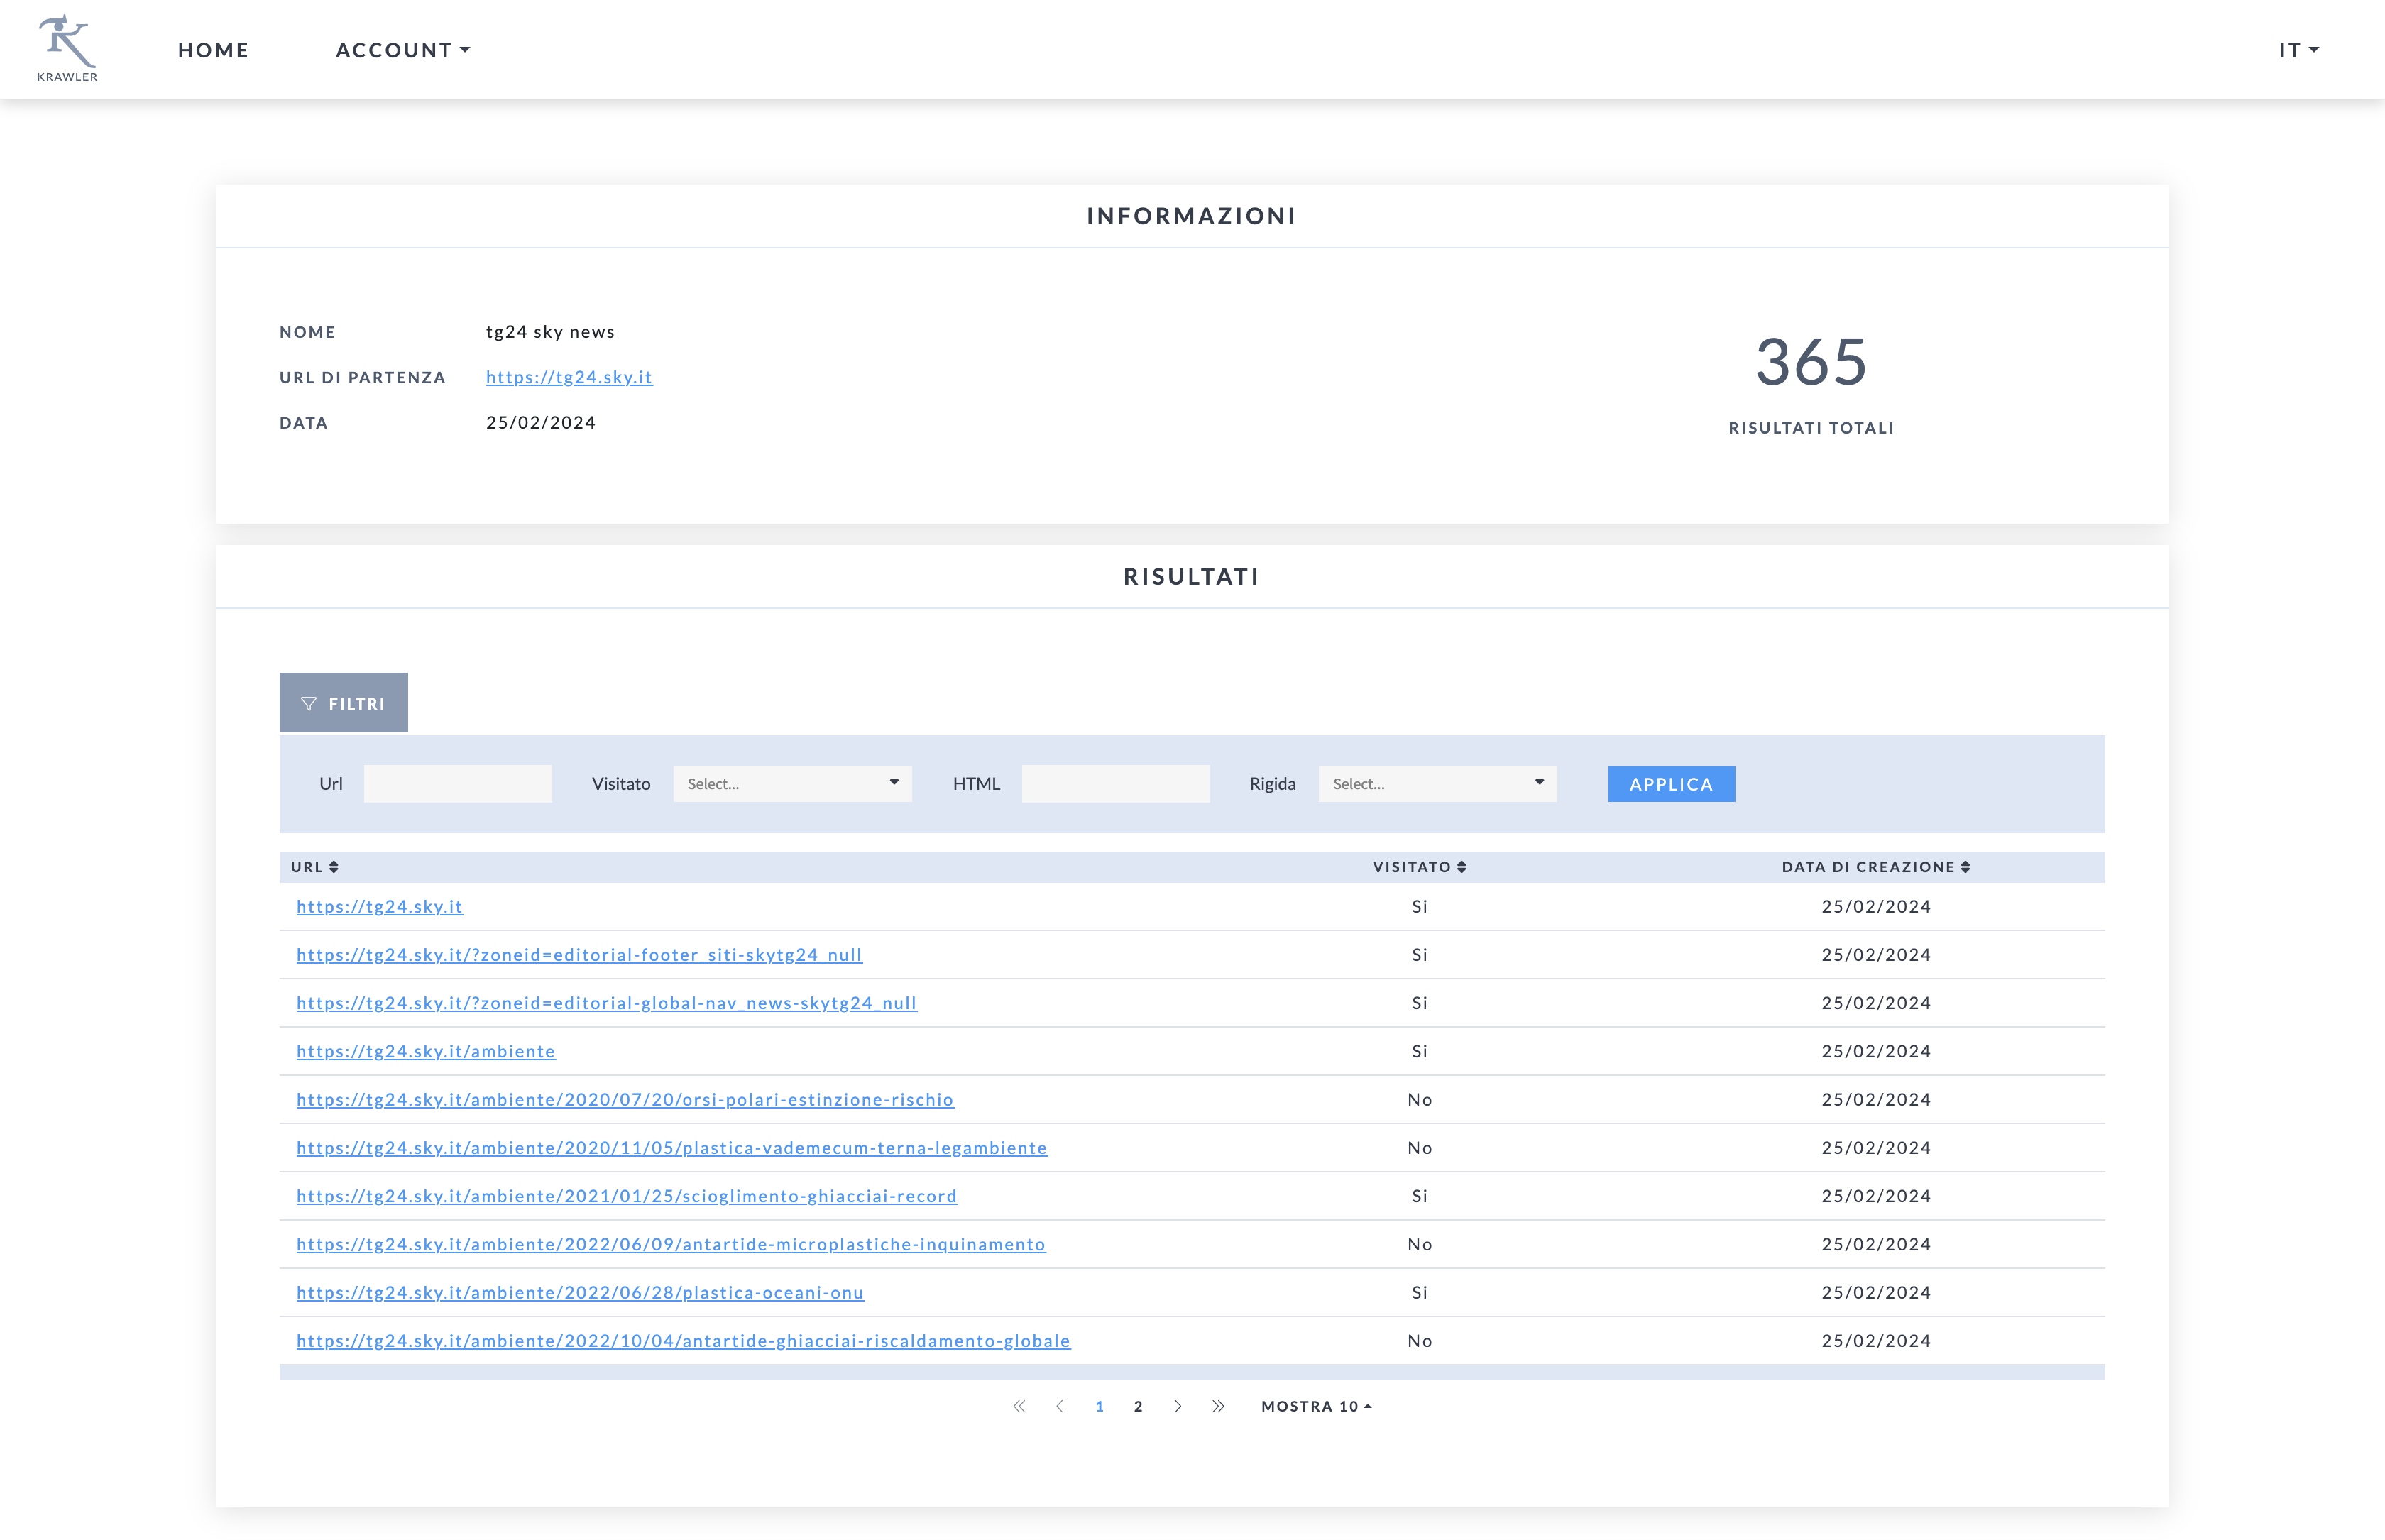
\includegraphics[width=1\textwidth]{appendix/frontend_search_details.png}
    \caption[View and filter results screen]{View and filter results of a specified search.}
    \label{fig:frontend_search_details}
\end{figure}

\begin{comment}
\begin{sidewaysfigure}[ht]
    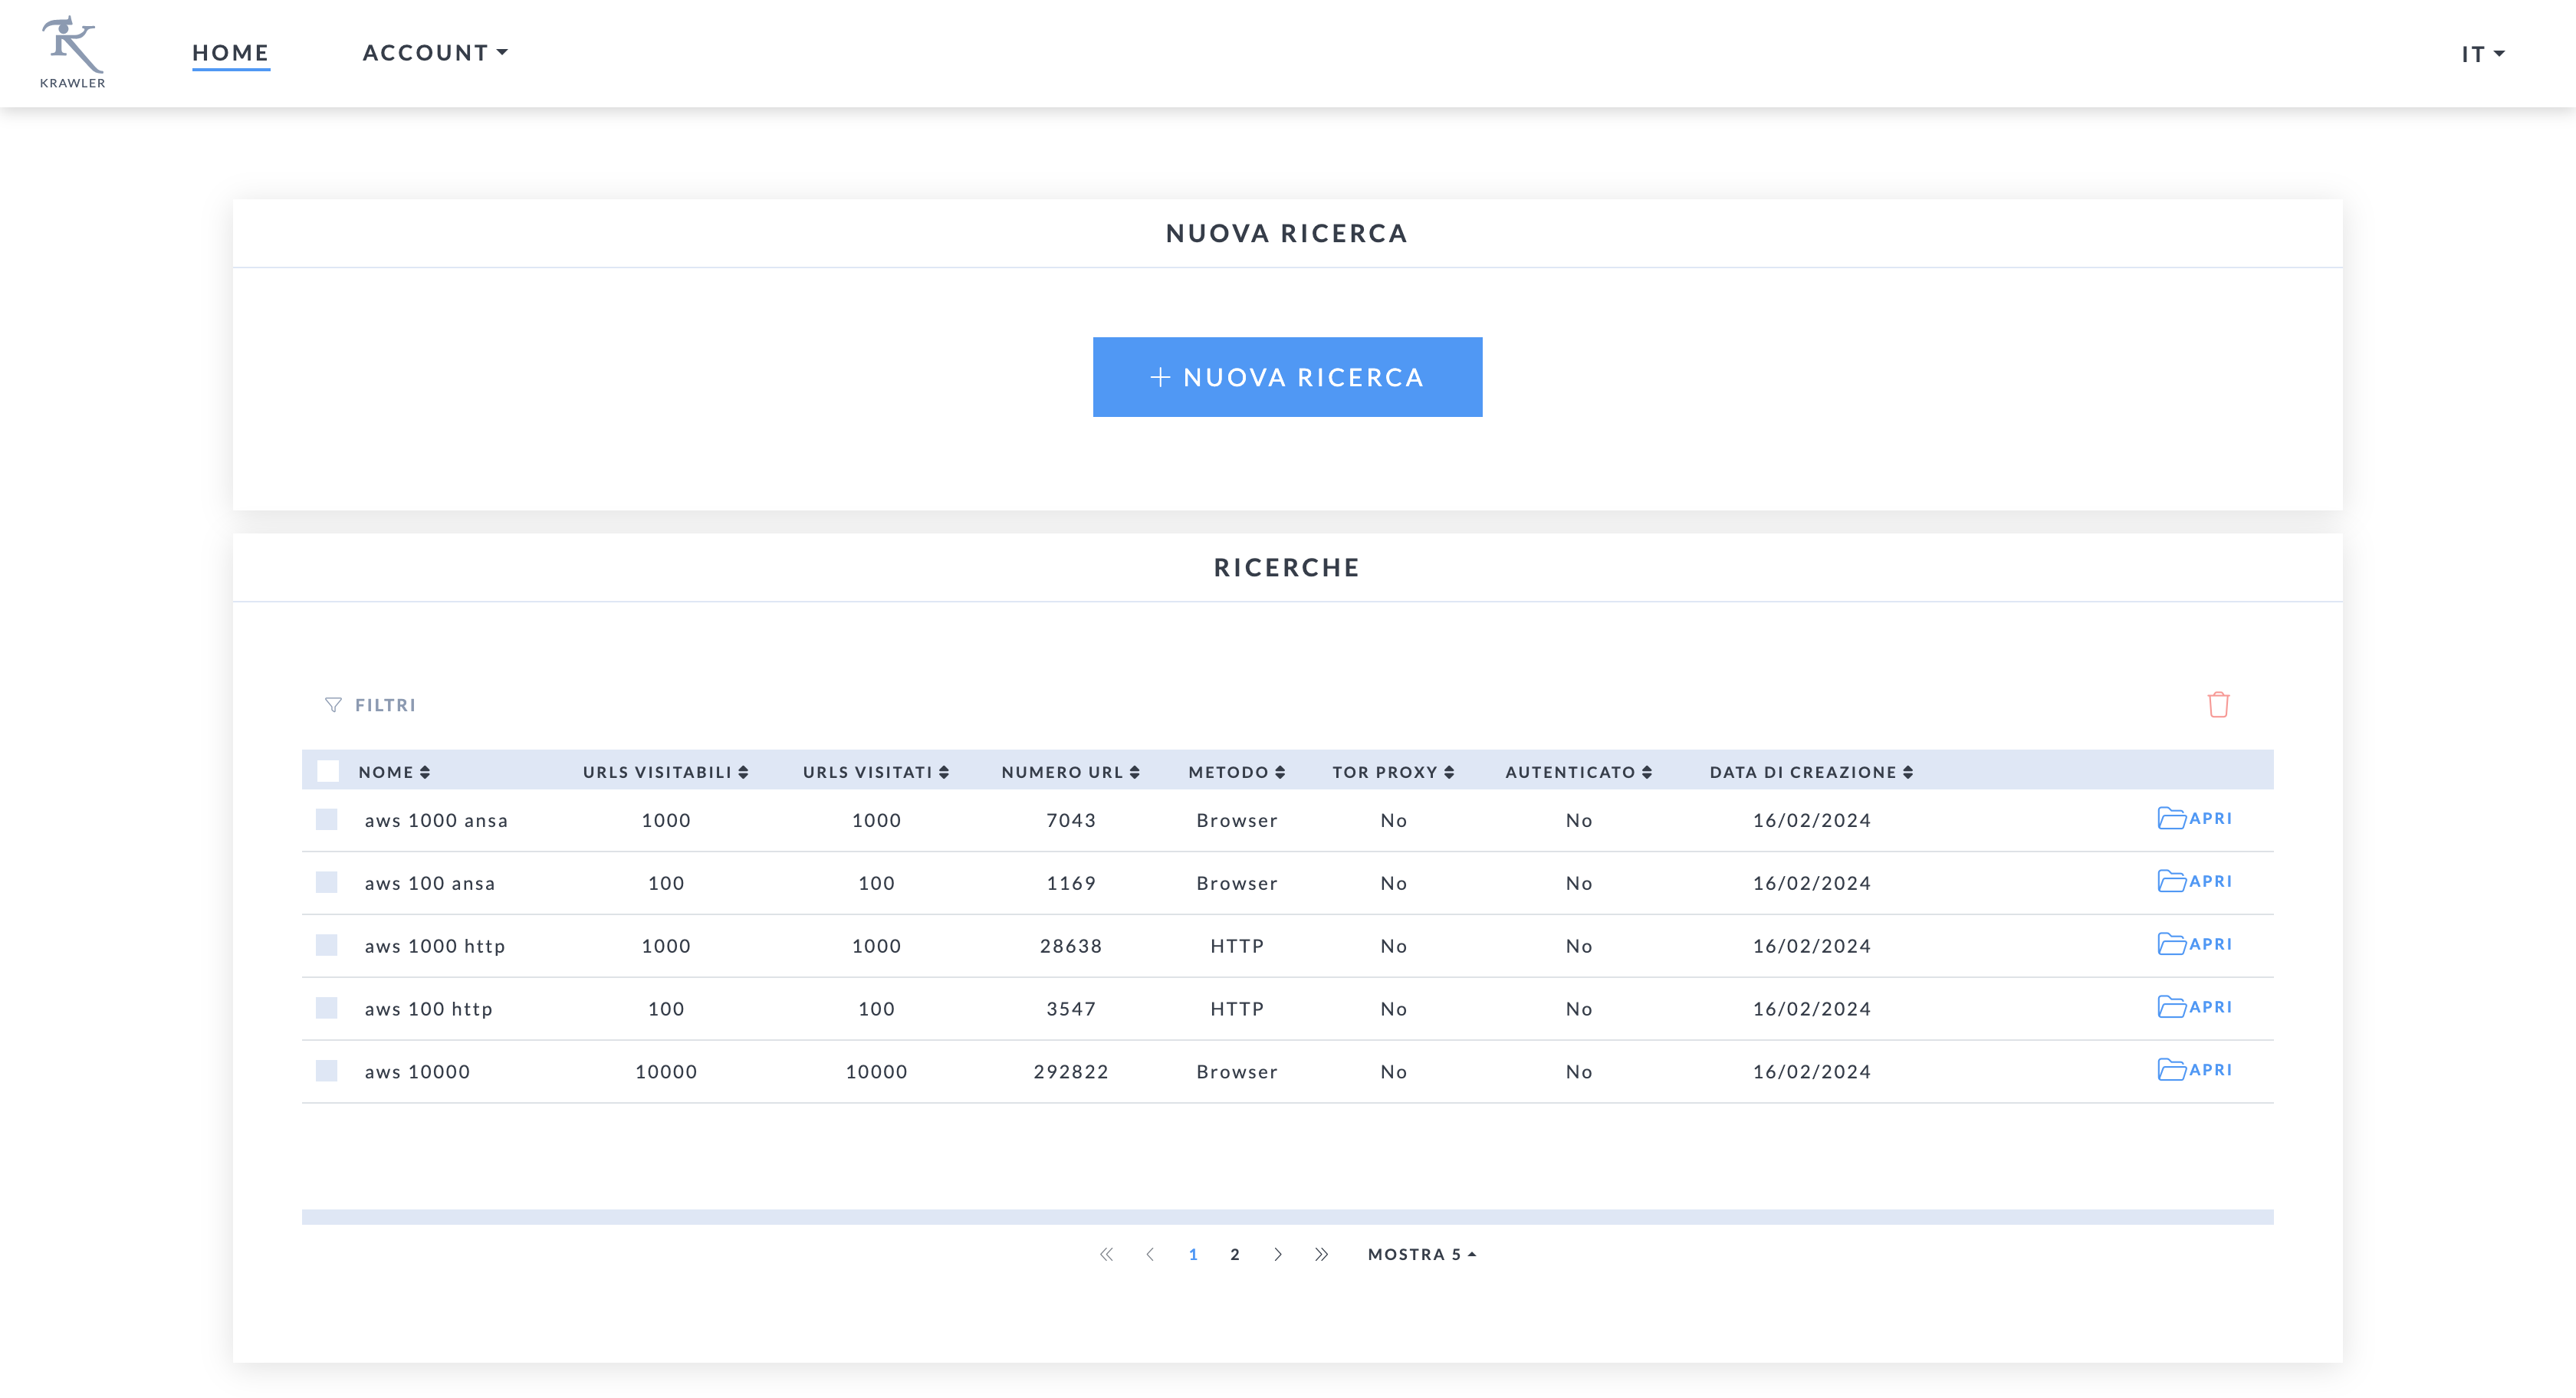
\includegraphics[width=1\textwidth]{appendix/frontend_dashboard.png}
    \caption[Dashboard screen]{Dashboard.}
    \label{fig:frontend_dashboard}
\end{sidewaysfigure}

\begin{sidewaysfigure}[ht]
    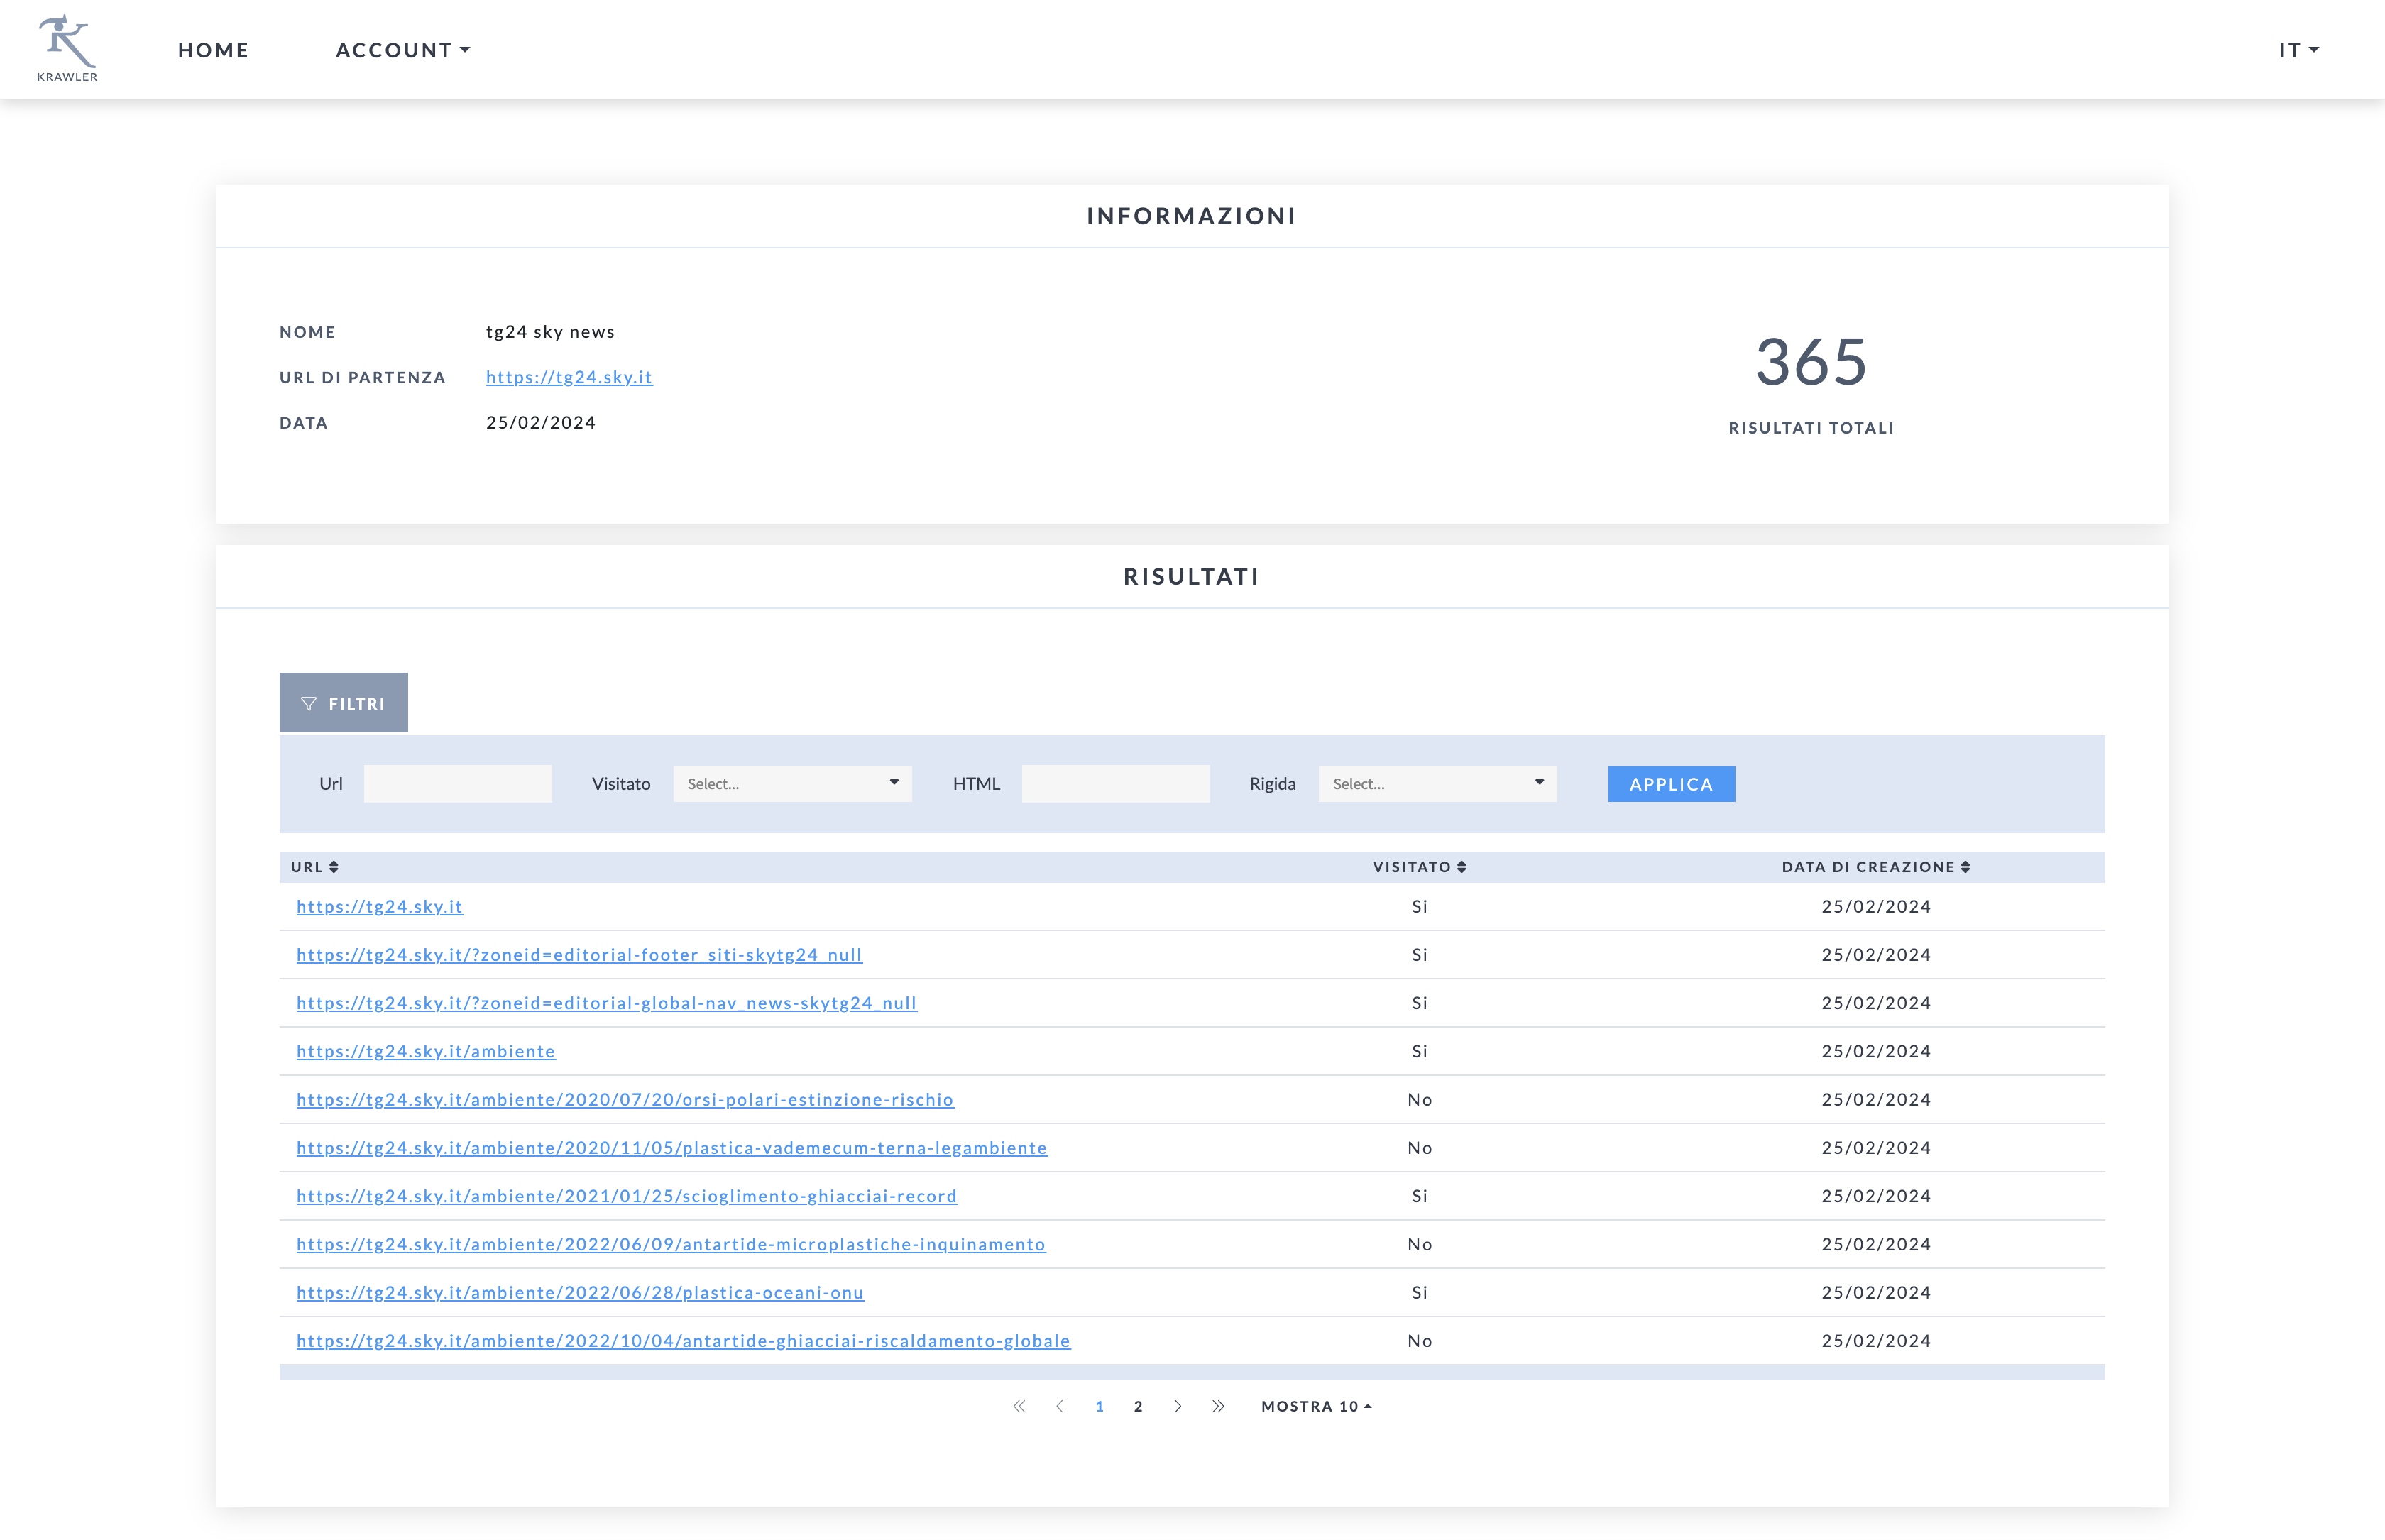
\includegraphics[width=1\textwidth]{appendix/frontend_search_details.png}
    \caption[View and filter results screen]{View and filter results of a specified search.}
    \label{fig:frontend_search_details}
\end{sidewaysfigure}

\begin{sidewaysfigure}[ht]
    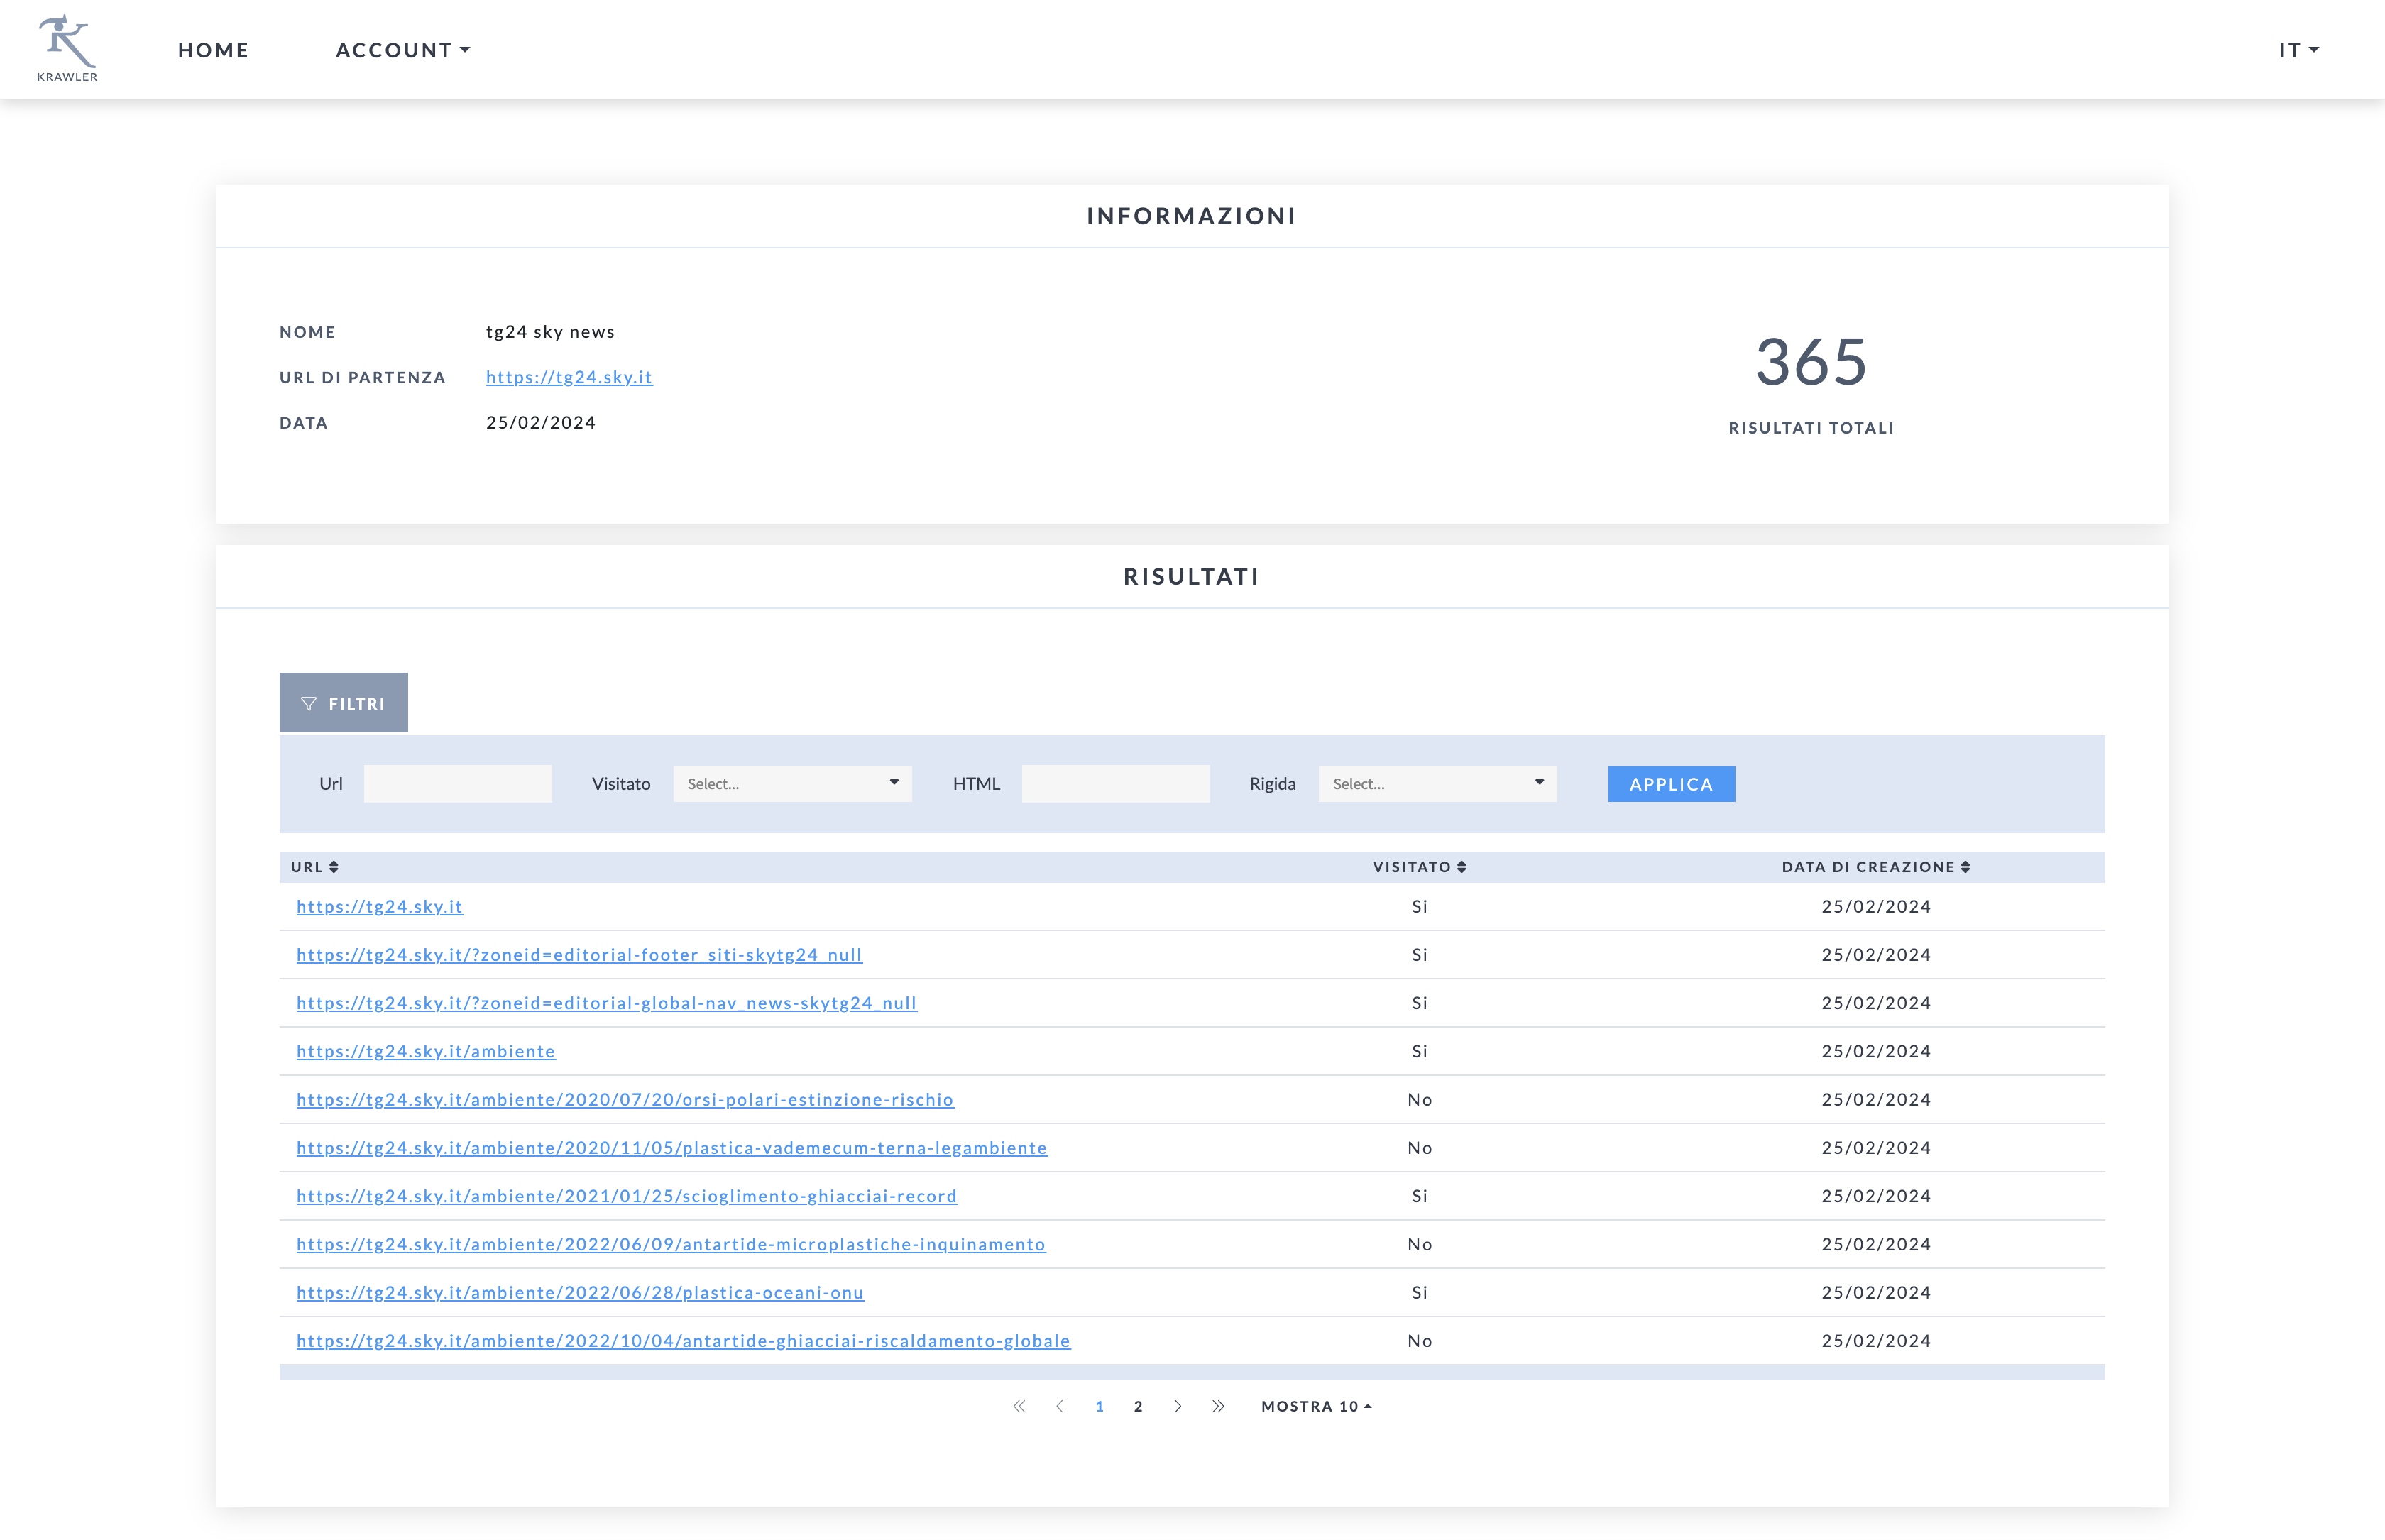
\includegraphics[width=1\textwidth]{appendix/frontend_search_details.png}
    \caption[View and filter results screen]{View and filter results of a specified search.}
    \label{fig:frontend_search_details}
\end{sidewaysfigure}
\end{comment}

\chapter{Configurations}
\section{Knative}\label{appendix:knative_conf}

The Knative implementation includes many commands to run and resources to deploy; therefore, all have been reported in this chapter.

In the \acrshort{YAML} files, a placeholder will be inserted when referring to the \textit{namespace} field, which must be replaced at your convenience.

\lstinputlisting[language=bash, captionpos=b, caption={[Deploy Knative stack through script]Bash script used to deploy Knative Serving, Eventing and RabbitMQ components.}, label={code:knative_install_script}]{ext_files/install-knative.sh}

\lstinputlisting[language=yaml, captionpos=b, caption={[Deploy a RabbitMQ cluster]How to deploy a RabbitMQ cluster.}, label={code:rabbitmq_cluster}]{ext_files/rabbitmq.yaml}

\lstinputlisting[language=yaml, captionpos=b, caption={[Deploy a RabbitMQ broker]How to deploy a RabbitMQ broker with its configuration.}, label={code:rabbitmq_broker}]{ext_files/broker.yaml}

\lstinputlisting[language=yaml, captionpos=b, caption={[Knative Service of event-display utility]Knative Service of event-display utility.}, label={code:event_display}]{ext_files/utility.yaml}

\lstinputlisting[language=yaml, captionpos=b, caption={[Knative Services of the backend module]Knative Services of the backend module.}, label={code:kn_kapturer_be}]{ext_files/backend.yaml}

\lstinputlisting[language=yaml, captionpos=b, caption={[Knative Services of the core module]Knative Services of the core module.}, label={code:kn_krawler}]{ext_files/function.yaml}

\lstinputlisting[language=yaml, captionpos=b, caption={[Trigger definitions]Trigger definitions to subscribe event to a sink.}, label={code:kn_trigger}]{ext_files/triggers.yaml}

\section{Monitoring}\label{appendix:monitoring_conf}

The collection and storage of metrics generated during the various tests was made possible by the monitoring platform, which includes several applications. The commands required for deploying and configuring the latter are listed below.

A complete reading of the configuration files is recommended before running any commands.

\lstinputlisting[language=bash, captionpos=b, caption={[How to deploy the monitoring stack]How to deploy Prometheus Stack, InfluxDB and Telegraf.}, label={code:monitoring_stack}]{ext_files/install-monitoring.sh}

\lstinputlisting[language=yaml, captionpos=b, caption={[Definition of prom-values.yaml]prom-values.yaml}, label={code:prom_values}]{ext_files/prom-values.yaml}

\lstinputlisting[language=yaml, captionpos=b, caption={[Definition of inf-values.yaml]inf-values.yaml}, label={code:inf_values}]{ext_files/inf-values.yaml}

\lstinputlisting[language=yaml, captionpos=b, caption={[Definition of tel-values.yaml]tel-values.yaml}, label={code:tel_values}]{ext_files/tel-values.yaml}

\end{document}